\hypertarget{stm32f4xx__hal__i2c_8c}{}\section{Dokumentacja pliku S\+T\+M/\+W\+D\+S\+\_\+\+Kosc\+\_\+\+Linux/\+Drivers/\+S\+T\+M32\+F4xx\+\_\+\+H\+A\+L\+\_\+\+Driver/\+Src/stm32f4xx\+\_\+hal\+\_\+i2c.c}
\label{stm32f4xx__hal__i2c_8c}\index{S\+T\+M/\+W\+D\+S\+\_\+\+Kosc\+\_\+\+Linux/\+Drivers/\+S\+T\+M32\+F4xx\+\_\+\+H\+A\+L\+\_\+\+Driver/\+Src/stm32f4xx\+\_\+hal\+\_\+i2c.\+c@{S\+T\+M/\+W\+D\+S\+\_\+\+Kosc\+\_\+\+Linux/\+Drivers/\+S\+T\+M32\+F4xx\+\_\+\+H\+A\+L\+\_\+\+Driver/\+Src/stm32f4xx\+\_\+hal\+\_\+i2c.\+c}}


I2C H\+AL module driver. This file provides firmware functions to manage the following functionalities of the Inter Integrated Circuit (I2C) peripheral\+:  


{\ttfamily \#include \char`\"{}stm32f4xx\+\_\+hal.\+h\char`\"{}}\newline
Wykres zależności załączania dla stm32f4xx\+\_\+hal\+\_\+i2c.\+c\+:\nopagebreak
\begin{figure}[H]
\begin{center}
\leavevmode
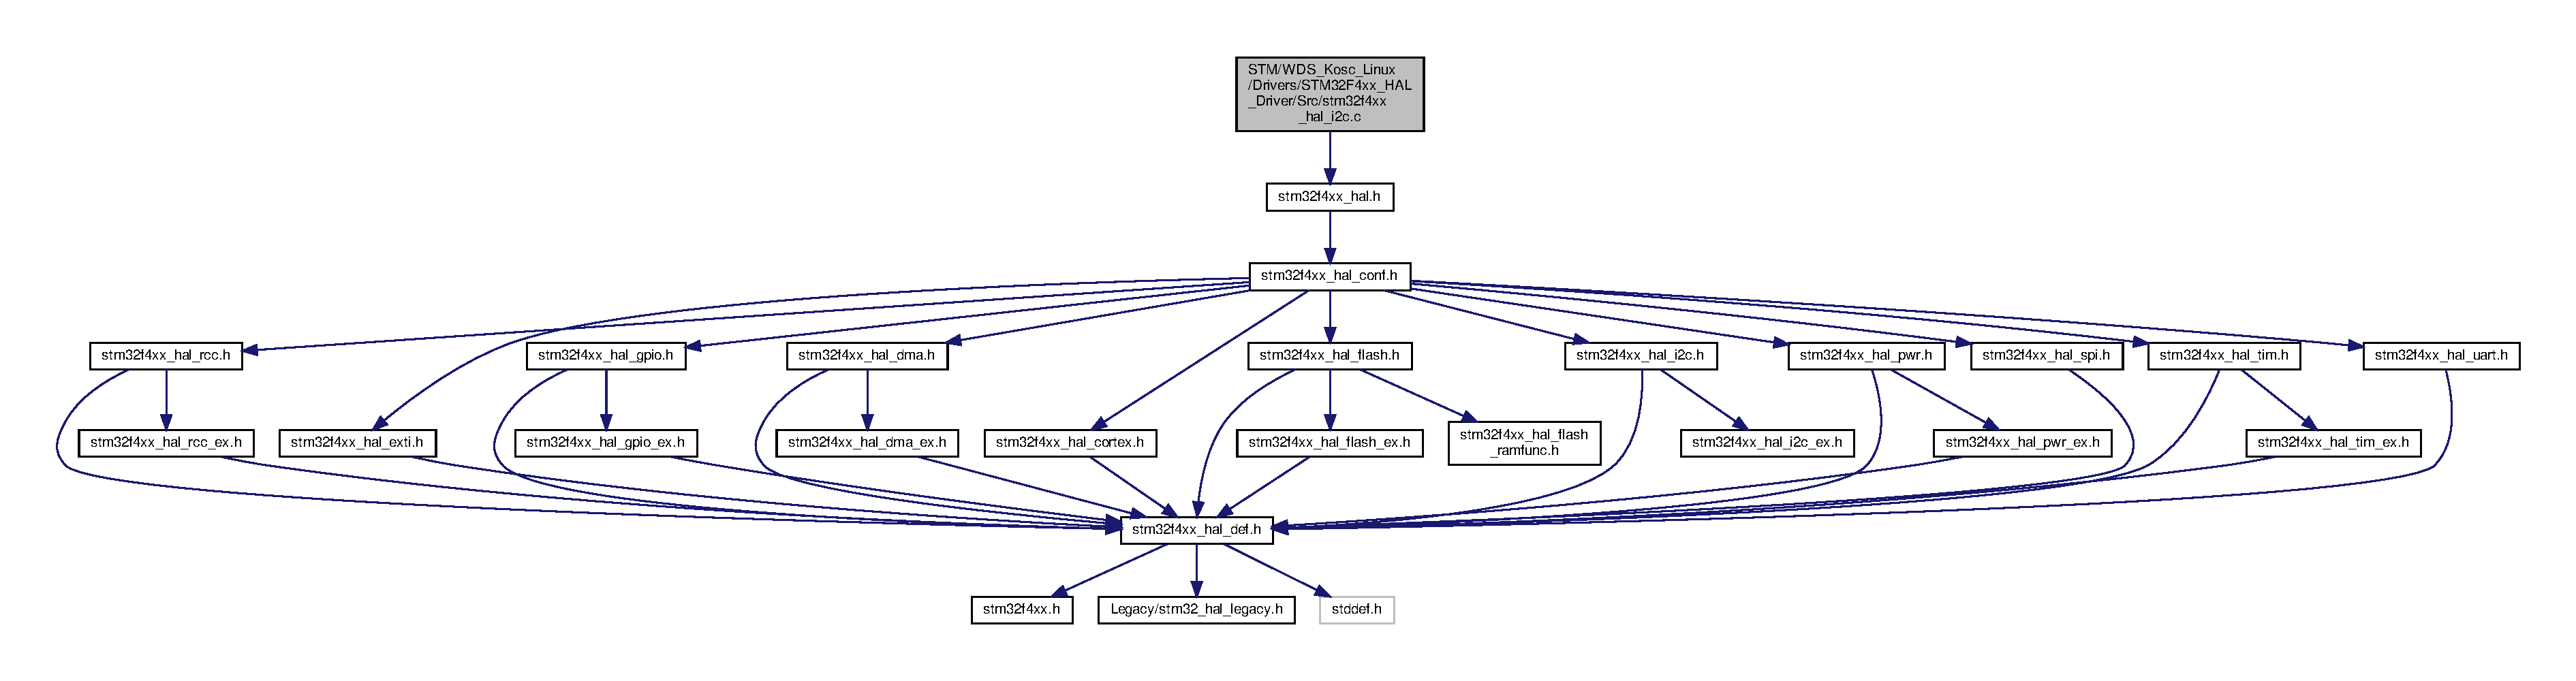
\includegraphics[width=350pt]{stm32f4xx__hal__i2c_8c__incl}
\end{center}
\end{figure}


\subsection{Opis szczegółowy}
I2C H\+AL module driver. This file provides firmware functions to manage the following functionalities of the Inter Integrated Circuit (I2C) peripheral\+: 

\begin{DoxyAuthor}{Autor}
M\+CD Application Team
\begin{DoxyItemize}
\item Initialization and de-\/initialization functions
\item IO operation functions
\item Peripheral State, Mode and Error functions
\end{DoxyItemize}
\end{DoxyAuthor}
\begin{DoxyVerb}==============================================================================
                      ##### How to use this driver #####
==============================================================================
[..]
  The I2C HAL driver can be used as follows:

  (#) Declare a I2C_HandleTypeDef handle structure, for example:
      I2C_HandleTypeDef  hi2c;

  (#)Initialize the I2C low level resources by implementing the @ref HAL_I2C_MspInit() API:
      (##) Enable the I2Cx interface clock
      (##) I2C pins configuration
          (+++) Enable the clock for the I2C GPIOs
          (+++) Configure I2C pins as alternate function open-drain
      (##) NVIC configuration if you need to use interrupt process
          (+++) Configure the I2Cx interrupt priority
          (+++) Enable the NVIC I2C IRQ Channel
      (##) DMA Configuration if you need to use DMA process
          (+++) Declare a DMA_HandleTypeDef handle structure for the transmit or receive stream
          (+++) Enable the DMAx interface clock using
          (+++) Configure the DMA handle parameters
          (+++) Configure the DMA Tx or Rx stream
          (+++) Associate the initialized DMA handle to the hi2c DMA Tx or Rx handle
          (+++) Configure the priority and enable the NVIC for the transfer complete interrupt on
                the DMA Tx or Rx stream

  (#) Configure the Communication Speed, Duty cycle, Addressing mode, Own Address1,
      Dual Addressing mode, Own Address2, General call and Nostretch mode in the hi2c Init structure.

  (#) Initialize the I2C registers by calling the @ref HAL_I2C_Init(), configures also the low level Hardware
      (GPIO, CLOCK, NVIC...etc) by calling the customized @ref HAL_I2C_MspInit() API.

  (#) To check if target device is ready for communication, use the function @ref HAL_I2C_IsDeviceReady()

  (#) For I2C IO and IO MEM operations, three operation modes are available within this driver :

  *** Polling mode IO operation ***
  =================================
  [..]
    (+) Transmit in master mode an amount of data in blocking mode using @ref HAL_I2C_Master_Transmit()
    (+) Receive in master mode an amount of data in blocking mode using @ref HAL_I2C_Master_Receive()
    (+) Transmit in slave mode an amount of data in blocking mode using @ref HAL_I2C_Slave_Transmit()
    (+) Receive in slave mode an amount of data in blocking mode using @ref HAL_I2C_Slave_Receive()

  *** Polling mode IO MEM operation ***
  =====================================
  [..]
    (+) Write an amount of data in blocking mode to a specific memory address using @ref HAL_I2C_Mem_Write()
    (+) Read an amount of data in blocking mode from a specific memory address using @ref HAL_I2C_Mem_Read()


  *** Interrupt mode IO operation ***
  ===================================
  [..]
    (+) Transmit in master mode an amount of data in non-blocking mode using @ref HAL_I2C_Master_Transmit_IT()
    (+) At transmission end of transfer, @ref HAL_I2C_MasterTxCpltCallback() is executed and user can
         add his own code by customization of function pointer @ref HAL_I2C_MasterTxCpltCallback()
    (+) Receive in master mode an amount of data in non-blocking mode using @ref HAL_I2C_Master_Receive_IT()
    (+) At reception end of transfer, @ref HAL_I2C_MasterRxCpltCallback() is executed and user can
         add his own code by customization of function pointer @ref HAL_I2C_MasterRxCpltCallback()
    (+) Transmit in slave mode an amount of data in non-blocking mode using @ref HAL_I2C_Slave_Transmit_IT()
    (+) At transmission end of transfer, @ref HAL_I2C_SlaveTxCpltCallback() is executed and user can
         add his own code by customization of function pointer @ref HAL_I2C_SlaveTxCpltCallback()
    (+) Receive in slave mode an amount of data in non-blocking mode using @ref HAL_I2C_Slave_Receive_IT()
    (+) At reception end of transfer, @ref HAL_I2C_SlaveRxCpltCallback() is executed and user can
         add his own code by customization of function pointer @ref HAL_I2C_SlaveRxCpltCallback()
    (+) In case of transfer Error, @ref HAL_I2C_ErrorCallback() function is executed and user can
         add his own code by customization of function pointer @ref HAL_I2C_ErrorCallback()
    (+) Abort a master I2C process communication with Interrupt using @ref HAL_I2C_Master_Abort_IT()
    (+) End of abort process, @ref HAL_I2C_AbortCpltCallback() is executed and user can
         add his own code by customization of function pointer @ref HAL_I2C_AbortCpltCallback()

  *** Interrupt mode or DMA mode IO sequential operation ***
  ==========================================================
  [..]
    (@) These interfaces allow to manage a sequential transfer with a repeated start condition
        when a direction change during transfer
  [..]
    (+) A specific option field manage the different steps of a sequential transfer
    (+) Option field values are defined through @ref I2C_XferOptions_definition and are listed below:
    (++) I2C_FIRST_AND_LAST_FRAME: No sequential usage, functionnal is same as associated interfaces in no sequential mode
    (++) I2C_FIRST_FRAME: Sequential usage, this option allow to manage a sequence with start condition, address
                          and data to transfer without a final stop condition
    (++) I2C_FIRST_AND_NEXT_FRAME: Sequential usage (Master only), this option allow to manage a sequence with start condition, address
                          and data to transfer without a final stop condition, an then permit a call the same master sequential interface
                          several times (like @ref HAL_I2C_Master_Seq_Transmit_IT() then @ref HAL_I2C_Master_Seq_Transmit_IT()
                          or @ref HAL_I2C_Master_Seq_Transmit_DMA() then @ref HAL_I2C_Master_Seq_Transmit_DMA())
    (++) I2C_NEXT_FRAME: Sequential usage, this option allow to manage a sequence with a restart condition, address
                          and with new data to transfer if the direction change or manage only the new data to transfer
                          if no direction change and without a final stop condition in both cases
    (++) I2C_LAST_FRAME: Sequential usage, this option allow to manage a sequance with a restart condition, address
                          and with new data to transfer if the direction change or manage only the new data to transfer
                          if no direction change and with a final stop condition in both cases
    (++) I2C_LAST_FRAME_NO_STOP: Sequential usage (Master only), this option allow to manage a restart condition after several call of the same master sequential
                          interface several times (link with option I2C_FIRST_AND_NEXT_FRAME).
                          Usage can, transfer several bytes one by one using HAL_I2C_Master_Seq_Transmit_IT(option I2C_FIRST_AND_NEXT_FRAME then I2C_NEXT_FRAME)
                            or HAL_I2C_Master_Seq_Receive_IT(option I2C_FIRST_AND_NEXT_FRAME then I2C_NEXT_FRAME)
                            or HAL_I2C_Master_Seq_Transmit_DMA(option I2C_FIRST_AND_NEXT_FRAME then I2C_NEXT_FRAME)
                            or HAL_I2C_Master_Seq_Receive_DMA(option I2C_FIRST_AND_NEXT_FRAME then I2C_NEXT_FRAME).
                          Then usage of this option I2C_LAST_FRAME_NO_STOP at the last Transmit or Receive sequence permit to call the oposite interface Receive or Transmit
                            without stopping the communication and so generate a restart condition.
    (++) I2C_OTHER_FRAME: Sequential usage (Master only), this option allow to manage a restart condition after each call of the same master sequential
                          interface.
                          Usage can, transfer several bytes one by one with a restart with slave address between each bytes using HAL_I2C_Master_Seq_Transmit_IT(option I2C_FIRST_FRAME then I2C_OTHER_FRAME)
                            or HAL_I2C_Master_Seq_Receive_IT(option I2C_FIRST_FRAME then I2C_OTHER_FRAME)
                            or HAL_I2C_Master_Seq_Transmit_DMA(option I2C_FIRST_FRAME then I2C_OTHER_FRAME)
                            or HAL_I2C_Master_Seq_Receive_DMA(option I2C_FIRST_FRAME then I2C_OTHER_FRAME).
                          Then usage of this option I2C_OTHER_AND_LAST_FRAME at the last frame to help automatic generation of STOP condition.

    (+) Differents sequential I2C interfaces are listed below:
    (++) Sequential transmit in master I2C mode an amount of data in non-blocking mode using @ref HAL_I2C_Master_Seq_Transmit_IT()
          or using @ref HAL_I2C_Master_Seq_Transmit_DMA()
    (+++) At transmission end of current frame transfer, @ref HAL_I2C_MasterTxCpltCallback() is executed and user can
         add his own code by customization of function pointer @ref HAL_I2C_MasterTxCpltCallback()
    (++) Sequential receive in master I2C mode an amount of data in non-blocking mode using @ref HAL_I2C_Master_Seq_Receive_IT()
          or using @ref HAL_I2C_Master_Seq_Receive_DMA()
    (+++) At reception end of current frame transfer, @ref HAL_I2C_MasterRxCpltCallback() is executed and user can
         add his own code by customization of function pointer @ref HAL_I2C_MasterRxCpltCallback()
    (++) Abort a master IT or DMA I2C process communication with Interrupt using @ref HAL_I2C_Master_Abort_IT()
    (+++) End of abort process, @ref HAL_I2C_AbortCpltCallback() is executed and user can
         add his own code by customization of function pointer @ref HAL_I2C_AbortCpltCallback()
    (++) Enable/disable the Address listen mode in slave I2C mode using @ref HAL_I2C_EnableListen_IT() @ref HAL_I2C_DisableListen_IT()
    (+++) When address slave I2C match, @ref HAL_I2C_AddrCallback() is executed and user can
         add his own code to check the Address Match Code and the transmission direction request by master (Write/Read).
    (+++) At Listen mode end @ref HAL_I2C_ListenCpltCallback() is executed and user can
         add his own code by customization of function pointer @ref HAL_I2C_ListenCpltCallback()
    (++) Sequential transmit in slave I2C mode an amount of data in non-blocking mode using @ref HAL_I2C_Slave_Seq_Transmit_IT()
          or using @ref HAL_I2C_Slave_Seq_Transmit_DMA()
    (+++) At transmission end of current frame transfer, @ref HAL_I2C_SlaveTxCpltCallback() is executed and user can
         add his own code by customization of function pointer @ref HAL_I2C_SlaveTxCpltCallback()
    (++) Sequential receive in slave I2C mode an amount of data in non-blocking mode using @ref HAL_I2C_Slave_Seq_Receive_IT()
          or using @ref HAL_I2C_Slave_Seq_Receive_DMA()
    (+++) At reception end of current frame transfer, @ref HAL_I2C_SlaveRxCpltCallback() is executed and user can
         add his own code by customization of function pointer @ref HAL_I2C_SlaveRxCpltCallback()
    (++) In case of transfer Error, @ref HAL_I2C_ErrorCallback() function is executed and user can
         add his own code by customization of function pointer @ref HAL_I2C_ErrorCallback()

  *** Interrupt mode IO MEM operation ***
  =======================================
  [..]
    (+) Write an amount of data in non-blocking mode with Interrupt to a specific memory address using
        @ref HAL_I2C_Mem_Write_IT()
    (+) At Memory end of write transfer, @ref HAL_I2C_MemTxCpltCallback() is executed and user can
         add his own code by customization of function pointer @ref HAL_I2C_MemTxCpltCallback()
    (+) Read an amount of data in non-blocking mode with Interrupt from a specific memory address using
        @ref HAL_I2C_Mem_Read_IT()
    (+) At Memory end of read transfer, @ref HAL_I2C_MemRxCpltCallback() is executed and user can
         add his own code by customization of function pointer @ref HAL_I2C_MemRxCpltCallback()
    (+) In case of transfer Error, @ref HAL_I2C_ErrorCallback() function is executed and user can
         add his own code by customization of function pointer @ref HAL_I2C_ErrorCallback()

  *** DMA mode IO operation ***
  ==============================
  [..]
    (+) Transmit in master mode an amount of data in non-blocking mode (DMA) using
        @ref HAL_I2C_Master_Transmit_DMA()
    (+) At transmission end of transfer, @ref HAL_I2C_MasterTxCpltCallback() is executed and user can
         add his own code by customization of function pointer @ref HAL_I2C_MasterTxCpltCallback()
    (+) Receive in master mode an amount of data in non-blocking mode (DMA) using
        @ref HAL_I2C_Master_Receive_DMA()
    (+) At reception end of transfer, @ref HAL_I2C_MasterRxCpltCallback() is executed and user can
         add his own code by customization of function pointer @ref HAL_I2C_MasterRxCpltCallback()
    (+) Transmit in slave mode an amount of data in non-blocking mode (DMA) using
        @ref HAL_I2C_Slave_Transmit_DMA()
    (+) At transmission end of transfer, @ref HAL_I2C_SlaveTxCpltCallback() is executed and user can
         add his own code by customization of function pointer @ref HAL_I2C_SlaveTxCpltCallback()
    (+) Receive in slave mode an amount of data in non-blocking mode (DMA) using
        @ref HAL_I2C_Slave_Receive_DMA()
    (+) At reception end of transfer, @ref HAL_I2C_SlaveRxCpltCallback() is executed and user can
         add his own code by customization of function pointer @ref HAL_I2C_SlaveRxCpltCallback()
    (+) In case of transfer Error, @ref HAL_I2C_ErrorCallback() function is executed and user can
         add his own code by customization of function pointer @ref HAL_I2C_ErrorCallback()
    (+) Abort a master I2C process communication with Interrupt using @ref HAL_I2C_Master_Abort_IT()
    (+) End of abort process, @ref HAL_I2C_AbortCpltCallback() is executed and user can
         add his own code by customization of function pointer @ref HAL_I2C_AbortCpltCallback()

  *** DMA mode IO MEM operation ***
  =================================
  [..]
    (+) Write an amount of data in non-blocking mode with DMA to a specific memory address using
        @ref HAL_I2C_Mem_Write_DMA()
    (+) At Memory end of write transfer, @ref HAL_I2C_MemTxCpltCallback() is executed and user can
         add his own code by customization of function pointer @ref HAL_I2C_MemTxCpltCallback()
    (+) Read an amount of data in non-blocking mode with DMA from a specific memory address using
        @ref HAL_I2C_Mem_Read_DMA()
    (+) At Memory end of read transfer, @ref HAL_I2C_MemRxCpltCallback() is executed and user can
         add his own code by customization of function pointer @ref HAL_I2C_MemRxCpltCallback()
    (+) In case of transfer Error, @ref HAL_I2C_ErrorCallback() function is executed and user can
         add his own code by customization of function pointer @ref HAL_I2C_ErrorCallback()


   *** I2C HAL driver macros list ***
   ==================================
   [..]
     Below the list of most used macros in I2C HAL driver.

    (+) @ref __HAL_I2C_ENABLE:     Enable the I2C peripheral
    (+) @ref __HAL_I2C_DISABLE:    Disable the I2C peripheral
    (+) @ref __HAL_I2C_GET_FLAG:   Checks whether the specified I2C flag is set or not
    (+) @ref __HAL_I2C_CLEAR_FLAG: Clear the specified I2C pending flag
    (+) @ref __HAL_I2C_ENABLE_IT:  Enable the specified I2C interrupt
    (+) @ref __HAL_I2C_DISABLE_IT: Disable the specified I2C interrupt

   *** Callback registration ***
   =============================================
  [..]
   The compilation flag USE_HAL_I2C_REGISTER_CALLBACKS when set to 1
   allows the user to configure dynamically the driver callbacks.
   Use Functions @ref HAL_I2C_RegisterCallback() or @ref HAL_I2C_RegisterAddrCallback()
   to register an interrupt callback.
  [..]
   Function @ref HAL_I2C_RegisterCallback() allows to register following callbacks:
     (+) MasterTxCpltCallback : callback for Master transmission end of transfer.
     (+) MasterRxCpltCallback : callback for Master reception end of transfer.
     (+) SlaveTxCpltCallback  : callback for Slave transmission end of transfer.
     (+) SlaveRxCpltCallback  : callback for Slave reception end of transfer.
     (+) ListenCpltCallback   : callback for end of listen mode.
     (+) MemTxCpltCallback    : callback for Memory transmission end of transfer.
     (+) MemRxCpltCallback    : callback for Memory reception end of transfer.
     (+) ErrorCallback        : callback for error detection.
     (+) AbortCpltCallback    : callback for abort completion process.
     (+) MspInitCallback      : callback for Msp Init.
     (+) MspDeInitCallback    : callback for Msp DeInit.
   This function takes as parameters the HAL peripheral handle, the Callback ID
   and a pointer to the user callback function.
  [..]
   For specific callback AddrCallback use dedicated register callbacks : @ref HAL_I2C_RegisterAddrCallback().
  [..]
   Use function @ref HAL_I2C_UnRegisterCallback to reset a callback to the default
   weak function.
   @ref HAL_I2C_UnRegisterCallback takes as parameters the HAL peripheral handle,
   and the Callback ID.
   This function allows to reset following callbacks:
     (+) MasterTxCpltCallback : callback for Master transmission end of transfer.
     (+) MasterRxCpltCallback : callback for Master reception end of transfer.
     (+) SlaveTxCpltCallback  : callback for Slave transmission end of transfer.
     (+) SlaveRxCpltCallback  : callback for Slave reception end of transfer.
     (+) ListenCpltCallback   : callback for end of listen mode.
     (+) MemTxCpltCallback    : callback for Memory transmission end of transfer.
     (+) MemRxCpltCallback    : callback for Memory reception end of transfer.
     (+) ErrorCallback        : callback for error detection.
     (+) AbortCpltCallback    : callback for abort completion process.
     (+) MspInitCallback      : callback for Msp Init.
     (+) MspDeInitCallback    : callback for Msp DeInit.
  [..]
   For callback AddrCallback use dedicated register callbacks : @ref HAL_I2C_UnRegisterAddrCallback().
  [..]
   By default, after the @ref HAL_I2C_Init() and when the state is @ref HAL_I2C_STATE_RESET
   all callbacks are set to the corresponding weak functions:
   examples @ref HAL_I2C_MasterTxCpltCallback(), @ref HAL_I2C_MasterRxCpltCallback().
   Exception done for MspInit and MspDeInit functions that are
   reset to the legacy weak functions in the @ref HAL_I2C_Init()/ @ref HAL_I2C_DeInit() only when
   these callbacks are null (not registered beforehand).
   If MspInit or MspDeInit are not null, the @ref HAL_I2C_Init()/ @ref HAL_I2C_DeInit()
   keep and use the user MspInit/MspDeInit callbacks (registered beforehand) whatever the state.
  [..]
   Callbacks can be registered/unregistered in @ref HAL_I2C_STATE_READY state only.
   Exception done MspInit/MspDeInit functions that can be registered/unregistered
   in @ref HAL_I2C_STATE_READY or @ref HAL_I2C_STATE_RESET state,
   thus registered (user) MspInit/DeInit callbacks can be used during the Init/DeInit.
   Then, the user first registers the MspInit/MspDeInit user callbacks
   using @ref HAL_I2C_RegisterCallback() before calling @ref HAL_I2C_DeInit()
   or @ref HAL_I2C_Init() function.
  [..]
   When the compilation flag USE_HAL_I2C_REGISTER_CALLBACKS is set to 0 or
   not defined, the callback registration feature is not available and all callbacks
   are set to the corresponding weak functions.



   [..]
     (@) You can refer to the I2C HAL driver header file for more useful macros\end{DoxyVerb}


\begin{DoxyAttention}{Uwaga}

\end{DoxyAttention}
\subsubsection*{\begin{center}\copyright{} Copyright (c) 2016 S\+T\+Microelectronics. All rights reserved.\end{center} }

This software component is licensed by ST under B\+SD 3-\/\+Clause license, the \char`\"{}\+License\char`\"{}; You may not use this file except in compliance with the License. You may obtain a copy of the License at\+: opensource.\+org/licenses/\+B\+S\+D-\/3-\/\+Clause 